%%%%%%%%%%%%%%%%%%%%%%%%%%%%%%%%%%%%%%%%%%%%%%%%%%%%%%%%%%%%%%%%%%%%%%%%%%%%%
% Баталов Семен, 2021                                                       %
%%%%%%%%%%%%%%%%%%%%%%%%%%%%%%%%%%%%%%%%%%%%%%%%%%%%%%%%%%%%%%%%%%%%%%%%%%%%%

\documentclass[12pt, a4paper]{article}
\usepackage[left=2.5cm, right=2.5cm, top=2.5cm, bottom=2.5cm]{geometry}
\usepackage[utf8]{inputenc}
\usepackage{graphicx}
\graphicspath{{./pictures/}}
\usepackage[english, russian]{babel}
\usepackage{indentfirst}
\usepackage{misccorr}
\usepackage{amsmath}

\title{Задача непрерывной классификации для Iris flower data set.}
\author{Баталов Семен}
\date{18.02.2021}

\begin{document}
    
    \sloppy
    
    \maketitle
    
    \section{Iris flower data set}
    
    Это стандартный набор данных, интегрированнный в модуль <<\textbf{sklearn}>> 
    языка <<\textbf{Python}>> (Рис.~\ref{image1}). Набор данных состоит из 150 
    образцов каждого из трех видов ириса (Iris setosa, Iris virginica и Iris 
    versicolor). Для каждого образца были измерены четыре характеристики: длина и 
    ширина чашелистиков и лепестков в сантиметрах. Основываясь на комбинации этих 
    четырех характеристик, можно разработать несложный классификатор, чтобы отличать 
    виды друг от друга.
    
    \begin{figure} [h]
        \center{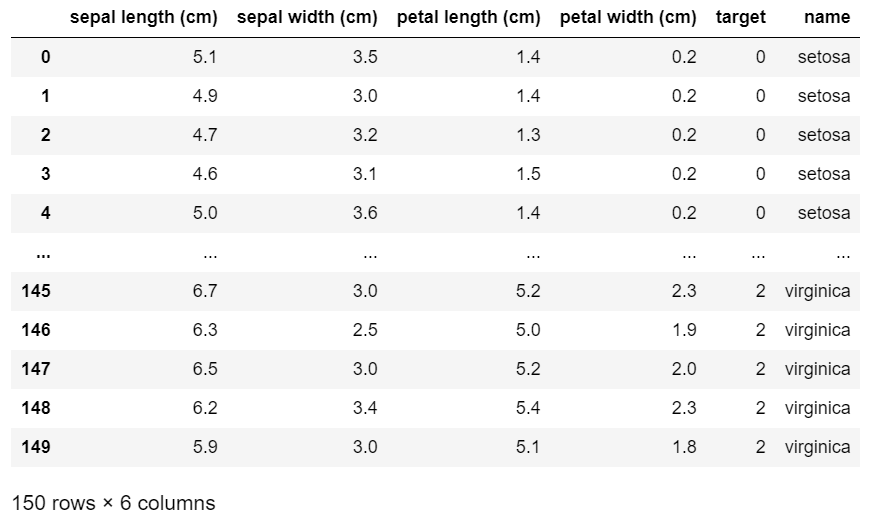
\includegraphics[width = 13cm]{iris_data_set.png}}
        \caption{Набор данных трех видов ириса.}
        \label{image1}
    \end{figure}
    
    \section{Классификаторы}
    
    Классификаторы были написан на языке <<\textbf{Python}>>. Подробнее о программе 
    можно узнать в папке <<\textbf{source}>> проекта. Было использовано два алгоритма 
    классификации: SVM (support vector machine), KNN (k-nearest neighbors algorithm). 
    Сначала рассмотрим алгоритм SVM.
    
    \subsection{Метод опорных векторов (SVM)}
    
    При написании программы использовался модуль <<\textbf{sklearn}>>, из него был 
    взят алгоритм <<\textbf{SupportVectorClassification}>>. Обучающая выборка 
    составила 50\% от всех полей (переставленных в случайном порядке) в наборе. 
    После была произведена проверка работоспособности классификатора на оставшихся в 
    датасете примерах. Результат проверки изображен на рисунке (Рис.~\ref{image2}).
    
    \begin{figure} [h]
        \center{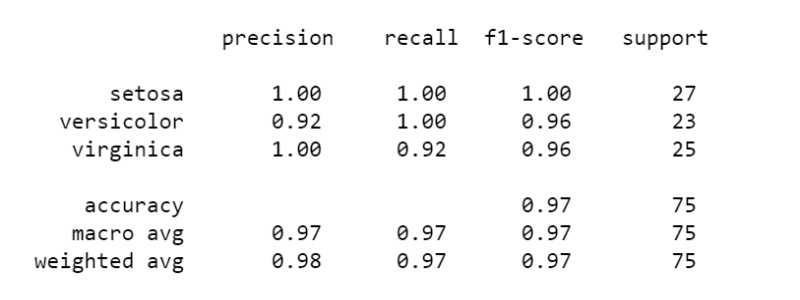
\includegraphics[width = 13cm]{result_SVM.png}}
        \caption{Оценка работы классификатора SVM.}
        \label{image2}
    \end{figure}
    
    \subsection{Метод <<k>> ближайших соседей (KNN)}
    
    При написании программы использовался модуль <<\textbf{sklearn}>>, из него был 
    взят алгоритм <<\textbf{KNeighborsClassifier}>>. Обучающая выборка составила 50\% 
    от всех полей (переставленных в случайном порядке) в наборе. После была 
    произведена проверка работоспособности классификатора на оставшихся в датасете 
    примерах. При этом количество соседей составило 10, а мера расстояния между 
    данными была стандартной евклидовой. Результат проверки изображен на рисунке 
    (Рис.~\ref{image3}).
    
    \begin{figure} [h]
        \center{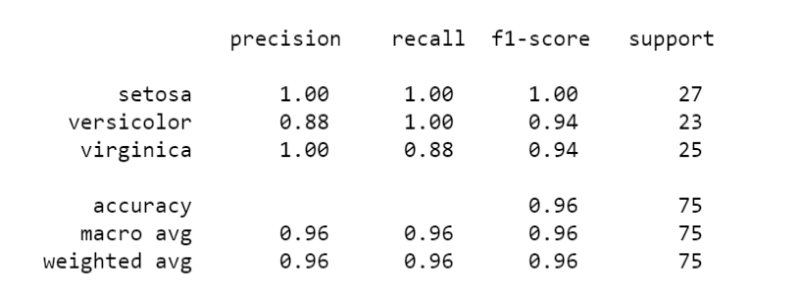
\includegraphics[width = 13cm]{result_KNN.png}}
        \caption{Оценка работы классификатора KNN.}
        \label{image3}
    \end{figure}
    
    Так же был произведен анализ того, какое количество соседей в данной задаче 
    является оптимальным. Для этого был использован алгоритм <<\textbf{k-fold 
    кросс-валидации}, идея которого заключается в разбиении всего набора данных на 
    <<k>> блоков схожих размеров. Далее поочередно один из этих блоков 
    используется как тестировочная выборка, а оставшиеся, как обучающая выборка, 
    производится обучение и анализ точности классификатора (под точность подразумеваем 
    отношение числа правильно классифицированных наборов данных к общему количеству 
    этих наборов). После этого из <<k>> независимых итераций обучения находится 
    среднее значение точности работы классификатора. В нашем случае эти значения 
    изображены на графике (Рис.~\ref{image4}).
    
    \begin{figure} [h]
        \center{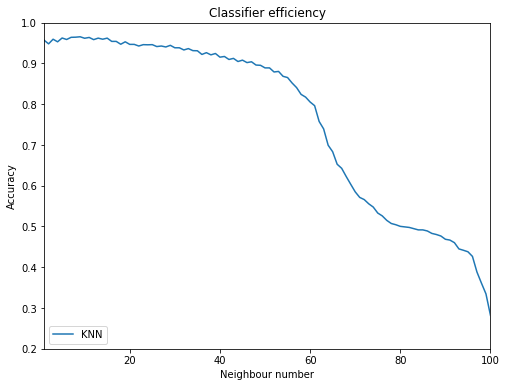
\includegraphics[width = 13cm]{accuracy_KNN.png}}
        \caption{График зависимости точности классификатора KNN от количества соседей.}
        \label{image4}
    \end{figure}
    
    Нетрудно видеть, что наилучший результат достигается при $k \in [2, \ldots, 15]$. 
    Более того, чем больше значение <<k>> тем хуже алгоритм справляется с задачей 
    классификации. В дальнейшем будем использовать (для эффективной работы) значение 
    <<k>> именно из описанного выше отрезка.
    
    \subsection{Сравнение SVM и KNN}
    
    Изучим, какой из алгоритмов на данном наборе данных лучше справляется с задачей 
    классификации. Для этого будем искать среднюю эффективность алгоритмов на 
    фиксированной обучающей и тестовой выборке. Стоит отметить, что выборки будут 
    использоваться с разным соотношением числа примеров для тренировки и для 
    тестировки. В алгоритме <<KNN>> будем брать $k \in [2, \ldots, 15]$. 
    
    Результаты обучения алгоритмов представлены на графике (Рис.~\ref{image5}). Здесь 
    число ближайших соседей равно 12.
    
    Видно, что при всех возможных выборках точность работы алгоритма <<SVM>> выше 
    точности алгоритма <<KNN>> (причем количество ближайших соседей выбрано 
    оптимальным). Также можно отметить, что точность у обоих подходов убывает при 
    сокращении количества обучающих примеров, но в методе <<KNN>> она убывает намного 
    быстрее.
    
    Можно сделать вывод, что оптимальное отношение количества примеров в обучающей и 
    тестировочной выборках к общему количеству примеров должно находиться в диапазоне 
    $[0,1 \ldots 0,4]$ для тестировочной и $[0,6 \ldots 0,9]$ для обучающей. 
    Критическим переходом можно считать соотношение $0.5$ для обеих выборок.
    
    \begin{figure} [h]
        \center{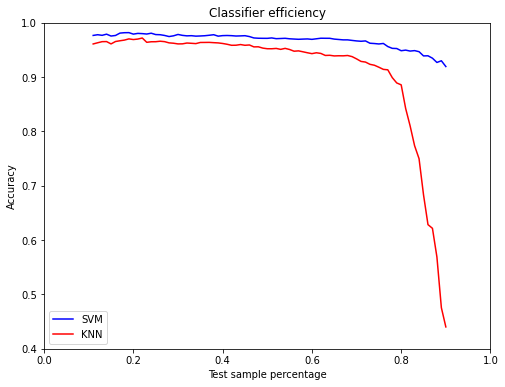
\includegraphics[width = 13cm]{comparison.png}}
        \caption{График зависимости точности классификаторов SVM и KNN от 
                 тестировочной выборки (и соответственно обучающей).}
        \label{image5}
    \end{figure}
    
\end{document}